% Options for packages loaded elsewhere
\PassOptionsToPackage{unicode}{hyperref}
\PassOptionsToPackage{hyphens}{url}
%
\documentclass[
]{article}
\usepackage{amsmath,amssymb}
\usepackage{iftex}
\ifPDFTeX
  \usepackage[T1]{fontenc}
  \usepackage[utf8]{inputenc}
  \usepackage{textcomp} % provide euro and other symbols
\else % if luatex or xetex
  \usepackage{unicode-math} % this also loads fontspec
  \defaultfontfeatures{Scale=MatchLowercase}
  \defaultfontfeatures[\rmfamily]{Ligatures=TeX,Scale=1}
\fi
\usepackage{lmodern}
\ifPDFTeX\else
  % xetex/luatex font selection
\fi
% Use upquote if available, for straight quotes in verbatim environments
\IfFileExists{upquote.sty}{\usepackage{upquote}}{}
\IfFileExists{microtype.sty}{% use microtype if available
  \usepackage[]{microtype}
  \UseMicrotypeSet[protrusion]{basicmath} % disable protrusion for tt fonts
}{}
\makeatletter
\@ifundefined{KOMAClassName}{% if non-KOMA class
  \IfFileExists{parskip.sty}{%
    \usepackage{parskip}
  }{% else
    \setlength{\parindent}{0pt}
    \setlength{\parskip}{6pt plus 2pt minus 1pt}}
}{% if KOMA class
  \KOMAoptions{parskip=half}}
\makeatother
\usepackage{xcolor}
\usepackage[margin=1in]{geometry}
\usepackage{color}
\usepackage{fancyvrb}
\newcommand{\VerbBar}{|}
\newcommand{\VERB}{\Verb[commandchars=\\\{\}]}
\DefineVerbatimEnvironment{Highlighting}{Verbatim}{commandchars=\\\{\}}
% Add ',fontsize=\small' for more characters per line
\usepackage{framed}
\definecolor{shadecolor}{RGB}{248,248,248}
\newenvironment{Shaded}{\begin{snugshade}}{\end{snugshade}}
\newcommand{\AlertTok}[1]{\textcolor[rgb]{0.94,0.16,0.16}{#1}}
\newcommand{\AnnotationTok}[1]{\textcolor[rgb]{0.56,0.35,0.01}{\textbf{\textit{#1}}}}
\newcommand{\AttributeTok}[1]{\textcolor[rgb]{0.13,0.29,0.53}{#1}}
\newcommand{\BaseNTok}[1]{\textcolor[rgb]{0.00,0.00,0.81}{#1}}
\newcommand{\BuiltInTok}[1]{#1}
\newcommand{\CharTok}[1]{\textcolor[rgb]{0.31,0.60,0.02}{#1}}
\newcommand{\CommentTok}[1]{\textcolor[rgb]{0.56,0.35,0.01}{\textit{#1}}}
\newcommand{\CommentVarTok}[1]{\textcolor[rgb]{0.56,0.35,0.01}{\textbf{\textit{#1}}}}
\newcommand{\ConstantTok}[1]{\textcolor[rgb]{0.56,0.35,0.01}{#1}}
\newcommand{\ControlFlowTok}[1]{\textcolor[rgb]{0.13,0.29,0.53}{\textbf{#1}}}
\newcommand{\DataTypeTok}[1]{\textcolor[rgb]{0.13,0.29,0.53}{#1}}
\newcommand{\DecValTok}[1]{\textcolor[rgb]{0.00,0.00,0.81}{#1}}
\newcommand{\DocumentationTok}[1]{\textcolor[rgb]{0.56,0.35,0.01}{\textbf{\textit{#1}}}}
\newcommand{\ErrorTok}[1]{\textcolor[rgb]{0.64,0.00,0.00}{\textbf{#1}}}
\newcommand{\ExtensionTok}[1]{#1}
\newcommand{\FloatTok}[1]{\textcolor[rgb]{0.00,0.00,0.81}{#1}}
\newcommand{\FunctionTok}[1]{\textcolor[rgb]{0.13,0.29,0.53}{\textbf{#1}}}
\newcommand{\ImportTok}[1]{#1}
\newcommand{\InformationTok}[1]{\textcolor[rgb]{0.56,0.35,0.01}{\textbf{\textit{#1}}}}
\newcommand{\KeywordTok}[1]{\textcolor[rgb]{0.13,0.29,0.53}{\textbf{#1}}}
\newcommand{\NormalTok}[1]{#1}
\newcommand{\OperatorTok}[1]{\textcolor[rgb]{0.81,0.36,0.00}{\textbf{#1}}}
\newcommand{\OtherTok}[1]{\textcolor[rgb]{0.56,0.35,0.01}{#1}}
\newcommand{\PreprocessorTok}[1]{\textcolor[rgb]{0.56,0.35,0.01}{\textit{#1}}}
\newcommand{\RegionMarkerTok}[1]{#1}
\newcommand{\SpecialCharTok}[1]{\textcolor[rgb]{0.81,0.36,0.00}{\textbf{#1}}}
\newcommand{\SpecialStringTok}[1]{\textcolor[rgb]{0.31,0.60,0.02}{#1}}
\newcommand{\StringTok}[1]{\textcolor[rgb]{0.31,0.60,0.02}{#1}}
\newcommand{\VariableTok}[1]{\textcolor[rgb]{0.00,0.00,0.00}{#1}}
\newcommand{\VerbatimStringTok}[1]{\textcolor[rgb]{0.31,0.60,0.02}{#1}}
\newcommand{\WarningTok}[1]{\textcolor[rgb]{0.56,0.35,0.01}{\textbf{\textit{#1}}}}
\usepackage{graphicx}
\makeatletter
\def\maxwidth{\ifdim\Gin@nat@width>\linewidth\linewidth\else\Gin@nat@width\fi}
\def\maxheight{\ifdim\Gin@nat@height>\textheight\textheight\else\Gin@nat@height\fi}
\makeatother
% Scale images if necessary, so that they will not overflow the page
% margins by default, and it is still possible to overwrite the defaults
% using explicit options in \includegraphics[width, height, ...]{}
\setkeys{Gin}{width=\maxwidth,height=\maxheight,keepaspectratio}
% Set default figure placement to htbp
\makeatletter
\def\fps@figure{htbp}
\makeatother
\setlength{\emergencystretch}{3em} % prevent overfull lines
\providecommand{\tightlist}{%
  \setlength{\itemsep}{0pt}\setlength{\parskip}{0pt}}
\setcounter{secnumdepth}{-\maxdimen} % remove section numbering
\usepackage{booktabs}
\usepackage{longtable}
\usepackage{array}
\usepackage{multirow}
\usepackage{wrapfig}
\usepackage{float}
\usepackage{colortbl}
\usepackage{pdflscape}
\usepackage{tabu}
\usepackage{threeparttable}
\usepackage{threeparttablex}
\usepackage[normalem]{ulem}
\usepackage{makecell}
\usepackage{xcolor}
\ifLuaTeX
  \usepackage{selnolig}  % disable illegal ligatures
\fi
\IfFileExists{bookmark.sty}{\usepackage{bookmark}}{\usepackage{hyperref}}
\IfFileExists{xurl.sty}{\usepackage{xurl}}{} % add URL line breaks if available
\urlstyle{same}
\hypersetup{
  pdftitle={ECON3032:   Statistical Estimation and Inference - Assignment},
  pdfauthor={Sammarieo Brown - ID: 620142596},
  hidelinks,
  pdfcreator={LaTeX via pandoc}}

\title{ECON3032: Statistical Estimation and Inference - Assignment}
\author{Sammarieo Brown - ID: 620142596}
\date{Friday, April 8, 2022 at 12pm}

\begin{document}
\maketitle

\hypertarget{method-of-moments-estimation---a-bootstrapping-study}{%
\subsubsection{Method of Moments Estimation - a Bootstrapping
Study}\label{method-of-moments-estimation---a-bootstrapping-study}}

{ The size of defaults on loans can be approximated by a gamma
distribution with shape parameter = \(\alpha = 1\) and the rate
parameter = \(\beta = 1/200\). The aim of this assignment is to use
bootstrapping to obtain the method of moments estimators
\(\hat{\alpha}_{MOM}\) and \(\hat{\beta}_{MOM}\).\\
}

{ 1. What type of distribution (discrete or continuous) is the amount of
a loan default? Explain your answer.}

The amount of a loan default is a continuous distribution. This is
because the size of defaults on loans can take on any value within a
continuous range, rather than being limited to a fixed set of discrete
values. In this case, the gamma distribution, which is a continuous
distribution, is used to approximate the size of loan defaults. The
gamma distribution is defined on the interval {[}0, ∞), which allows for
a wide range of possible loan default amounts.

\begin{Shaded}
\begin{Highlighting}[]
\FunctionTok{rm}\NormalTok{(}\AttributeTok{list =} \FunctionTok{ls}\NormalTok{()) }\CommentTok{\# Clear work environment}

\CommentTok{\# Set Working Directory}
\CommentTok{\#setwd("\textasciitilde{}/ECON3032/Assignment")}

\CommentTok{\# Load the Necessary Libraries}
\FunctionTok{library}\NormalTok{(psych) }\CommentTok{\# gives complete summary table}

\FunctionTok{library}\NormalTok{(kableExtra) }\CommentTok{\# for nice html table}

\FunctionTok{library}\NormalTok{(ggplot2) }\CommentTok{\# gives nice plots}

\FunctionTok{library}\NormalTok{(MASS) }\CommentTok{\# gives fits of density parameters}

\FunctionTok{library}\NormalTok{(EnvStats) }\CommentTok{\# for coefficient of variation}
\end{Highlighting}
\end{Shaded}

\begin{Shaded}
\begin{Highlighting}[]
\CommentTok{\# Import the original file}
\NormalTok{LoanDefaults }\OtherTok{\textless{}{-}} \FunctionTok{read.csv}\NormalTok{(}\StringTok{"E:/DataSpell/Statistical Computing Project/ECON3032 Assignment/LoanDefaults.csv"}\NormalTok{)}
\end{Highlighting}
\end{Shaded}

{ 2. Before beginning the study, calculate the mean and standard
deviation of the original dataset.}

\begin{Shaded}
\begin{Highlighting}[]
\FunctionTok{kable}\NormalTok{(}\FunctionTok{round}\NormalTok{(}\FunctionTok{describe}\NormalTok{(LoanDefaults[,}\DecValTok{2}\NormalTok{]), }\DecValTok{3}\NormalTok{)) }\SpecialCharTok{\%\textgreater{}\%}
  \FunctionTok{kable\_styling}\NormalTok{(}\AttributeTok{bootstrap\_options =} \FunctionTok{c}\NormalTok{(}\StringTok{"striped"}\NormalTok{, }\StringTok{"hover"}\NormalTok{), }\AttributeTok{full\_width =}\NormalTok{ F)}
\end{Highlighting}
\end{Shaded}

\begin{table}
\centering
\begin{tabular}{l|r|r|r|r|r|r|r|r|r|r|r|r|r}
\hline
  & vars & n & mean & sd & median & trimmed & mad & min & max & range & skew & kurtosis & se\\
\hline
X1 & 1 & 2e+05 & 199.759 & 199.212 & 138.875 & 166.048 & 142.597 & 0.002 & 2209.943 & 2209.941 & 1.986 & 5.857 & 0.445\\
\hline
\end{tabular}
\end{table}

{ 3. Get the parameters for the original distribution. Do the estimated
parameters seem to match the distribution in the introduction? Give
reasons for your answer. }

\begin{Shaded}
\begin{Highlighting}[]
\NormalTok{LoanDefault.Vec }\OtherTok{\textless{}{-}}\NormalTok{ LoanDefaults}\SpecialCharTok{$}\NormalTok{x}
\NormalTok{fit.params }\OtherTok{\textless{}{-}} \FunctionTok{fitdistr}\NormalTok{(LoanDefault.Vec,}\StringTok{"gamma"}\NormalTok{)  }\CommentTok{\# gives the maximum likelihood parameter estimates based on the distribution }
\NormalTok{fit.params}
\end{Highlighting}
\end{Shaded}

\begin{verbatim}
##       shape           rate    
##   1.003452e+00   5.023309e-03 
##  (2.738722e-03) (1.721828e-05)
\end{verbatim}

The estimated parameters for the original distribution are obtained
using the fitdistr() function from the MASS library, which provides the
maximum likelihood parameter estimates for the gamma distribution. The
estimated parameters are:

\begin{enumerate}
\def\labelenumi{\arabic{enumi}.}
\tightlist
\item
  Shape (α): 1.003452e+00 (approximately 1)
\item
  Rate (β): 5.023309e-03 (approximately 1/200)
\item
  These estimated parameters seem to match the distribution described in
  the introduction, where the shape parameter (α) is 1 and the rate
  parameter (β) is 1/200. The slight differences between the estimated
  parameters and the original distribution parameters can be attributed
  to sampling variability and the method used for estimation (maximum
  likelihood estimation in this case). Overall, the estimated parameters
  are close to the original distribution parameters, which suggests that
  the gamma distribution with these parameters is an appropriate model
  for the loan default data.
\end{enumerate}

\begin{Shaded}
\begin{Highlighting}[]
\CommentTok{\# Set the sampling seed for reproducibility}
\FunctionTok{set.seed}\NormalTok{(}\DecValTok{1300}\NormalTok{)}
\end{Highlighting}
\end{Shaded}

\begin{Shaded}
\begin{Highlighting}[]
\CommentTok{\# Select a random sample of data points from the original dataset}
\NormalTok{Loan.data }\OtherTok{\textless{}{-}}\NormalTok{ LoanDefaults[}\FunctionTok{sample}\NormalTok{(}\FunctionTok{nrow}\NormalTok{(LoanDefaults), }\DecValTok{67000}\NormalTok{), ]}

\NormalTok{Loan.data.Vec }\OtherTok{\textless{}{-}}\NormalTok{ Loan.data}\SpecialCharTok{$}\NormalTok{x}
\NormalTok{den }\OtherTok{\textless{}{-}} \FunctionTok{density}\NormalTok{(Loan.data.Vec)}
\NormalTok{dat }\OtherTok{\textless{}{-}} \FunctionTok{data.frame}\NormalTok{(}\AttributeTok{x =}\NormalTok{ den}\SpecialCharTok{$}\NormalTok{x, }\AttributeTok{y=}\NormalTok{ den}\SpecialCharTok{$}\NormalTok{y)}
\end{Highlighting}
\end{Shaded}

{ 4. Plot the data along with superimposed density curve. How well do
you think your data (the points in black) fit the assumed density curve
(the line in red)? }

\begin{Shaded}
\begin{Highlighting}[]
\NormalTok{h }\OtherTok{\textless{}{-}} \FunctionTok{hist}\NormalTok{(Loan.data.Vec, }\DecValTok{150}\NormalTok{, }\AttributeTok{plot=}\ConstantTok{FALSE}\NormalTok{)}
\NormalTok{t1 }\OtherTok{\textless{}{-}} \FunctionTok{data.frame}\NormalTok{(}\AttributeTok{x =}\NormalTok{ h}\SpecialCharTok{$}\NormalTok{mids, }\AttributeTok{y =}\NormalTok{ h}\SpecialCharTok{$}\NormalTok{density)}

\FunctionTok{ggplot}\NormalTok{(}\AttributeTok{data =}\NormalTok{ t1, }\FunctionTok{aes}\NormalTok{(}\AttributeTok{x =}\NormalTok{ x, }\AttributeTok{y =}\NormalTok{ y)) }\SpecialCharTok{+} 
  \FunctionTok{geom\_point}\NormalTok{(}\AttributeTok{size =} \DecValTok{3}\NormalTok{) }\SpecialCharTok{+}
  \FunctionTok{geom\_line}\NormalTok{(}\FunctionTok{aes}\NormalTok{(}\AttributeTok{x=}\NormalTok{x, }\AttributeTok{y=}\FunctionTok{dgamma}\NormalTok{(x,}\DecValTok{1}\NormalTok{, }\FloatTok{0.005}\NormalTok{)), }\AttributeTok{color=}\StringTok{"red"}\NormalTok{, }\AttributeTok{size =} \DecValTok{1}\NormalTok{) }\SpecialCharTok{+} 
  \FunctionTok{theme\_classic}\NormalTok{()}
\end{Highlighting}
\end{Shaded}

\begin{verbatim}
## Warning: Using `size` aesthetic for lines was deprecated in ggplot2 3.4.0.
## i Please use `linewidth` instead.
\end{verbatim}

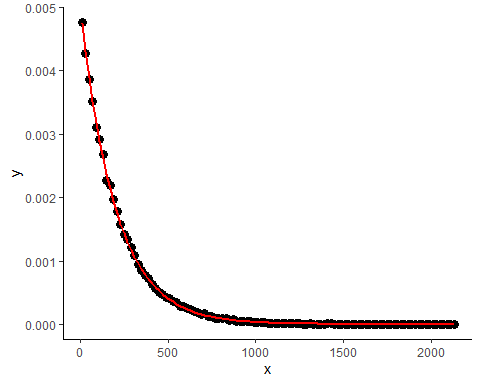
\includegraphics{Assignment_files/figure-latex/unnamed-chunk-7-1.pdf}

Based on the plot with the data points in black and the superimposed
density curve in red, it appears that the data fits the assumed gamma
density curve quite well. The distribution of the data points closely
follows the shape of the red density curve, suggesting that the gamma
distribution with the given shape and rate parameters is an appropriate
model for the loan default data.

4. The method of moments estimators for the parameters of the gamma
distribution are given as follows:

\[\begin{equation}
 \hat{\beta}_{MOM} = \dfrac{\bar{X}}{\dfrac{1}{n}\sum{_{i = 1}^{n}  X_i^2} - (\bar{X})^2}
\end{equation}\]

{ and}

\[\begin{equation}
 \hat{\alpha}_{MOM} =   \dfrac{(\bar{X})^2}{\dfrac{1}{n}\sum{_{i = 1}^{n}  X_i^2} - (\bar{X})^2} = \hat{\beta}_{MOM} \bar{X}
\end{equation}\]

{ To investigate the method of moments estimators, draw x number of
samples of size y and calculate \(\bar{X}\) and
\(\dfrac{1}{n}\sum{_{i = 1}^{n} X_i^2}\).}

\begin{Shaded}
\begin{Highlighting}[]
\CommentTok{\# Set up the vector to hold the values of xbar and sum of x\^{}2 divided by n}

\NormalTok{xbar }\OtherTok{\textless{}{-}} \FunctionTok{rep}\NormalTok{(}\DecValTok{0}\NormalTok{,}\DecValTok{2500}\NormalTok{)}
\NormalTok{x2bar }\OtherTok{\textless{}{-}} \FunctionTok{rep}\NormalTok{(}\DecValTok{0}\NormalTok{,}\DecValTok{2500}\NormalTok{)}


\CommentTok{\# Draw repeated samples from the dataset and calculate the estimators {-} This is called a For Loop}
\ControlFlowTok{for}\NormalTok{ (i }\ControlFlowTok{in} \DecValTok{1}\SpecialCharTok{:}\DecValTok{2500}\NormalTok{)\{}
\NormalTok{  xx }\OtherTok{\textless{}{-}} \FunctionTok{sample}\NormalTok{(LoanDefault.Vec, }\AttributeTok{size =} \DecValTok{2600}\NormalTok{, }\AttributeTok{replace =} \ConstantTok{FALSE}\NormalTok{)}
\NormalTok{  xbar[i]}\OtherTok{\textless{}{-}}\FunctionTok{mean}\NormalTok{(xx)}
\NormalTok{  x2bar[i]}\OtherTok{\textless{}{-}}\FunctionTok{mean}\NormalTok{(xx}\SpecialCharTok{\^{}}\DecValTok{2}\NormalTok{)}
\NormalTok{  \}}
\end{Highlighting}
\end{Shaded}

{ 5. For each sample, calculate \(\hat{\alpha}_{MOM}\) and
\(\hat{\beta}_{MOM}\)}.

\begin{Shaded}
\begin{Highlighting}[]
\NormalTok{betahat }\OtherTok{\textless{}{-}}\NormalTok{ xbar}\SpecialCharTok{/}\NormalTok{(x2bar}\SpecialCharTok{{-}}\NormalTok{xbar}\SpecialCharTok{\^{}}\DecValTok{2}\NormalTok{)}
\NormalTok{alphahat }\OtherTok{\textless{}{-}}\NormalTok{ betahat}\SpecialCharTok{*}\NormalTok{xbar}
\end{Highlighting}
\end{Shaded}

{ 6. Without doing any calculations, what should be the values of
\(\hat{\alpha}_{MOM}\) and \(\hat{\beta}_{MOM}\)? Given reasons for your
answer.}.

The values of α\^{}MOM and β\^{}MOM should be close to the true
parameters of the gamma distribution, which were provided in the
introduction. This is because the method of moments estimators aims to
match the moments of the sample with the moments of the distribution,
resulting in estimators that approximate the true distribution
parameters.

In this case, the true shape parameter (α) is 1, and the true rate
parameter (β) is 1/200. Therefore, we would expect the method of moments
estimators α\^{}MOM and β\^{}MOM to be close to these values. Keep in
mind that the estimators may not exactly match the true parameters due
to sampling variability, but they should provide a reasonable
approximation.

{ 7. Calculate the summary statistics for each estimator.}.

Summary Statistics for \(\hat{\beta}\)

\begin{Shaded}
\begin{Highlighting}[]
\FunctionTok{kable}\NormalTok{(}\FunctionTok{round}\NormalTok{(}\FunctionTok{describe}\NormalTok{(betahat), }\DecValTok{3}\NormalTok{)) }\SpecialCharTok{\%\textgreater{}\%}
  \FunctionTok{kable\_styling}\NormalTok{(}\AttributeTok{bootstrap\_options =} \FunctionTok{c}\NormalTok{(}\StringTok{"striped"}\NormalTok{, }\StringTok{"hover"}\NormalTok{), }\AttributeTok{full\_width =}\NormalTok{ F)}
\end{Highlighting}
\end{Shaded}

\begin{table}
\centering
\begin{tabular}{l|r|r|r|r|r|r|r|r|r|r|r|r|r}
\hline
  & vars & n & mean & sd & median & trimmed & mad & min & max & range & skew & kurtosis & se\\
\hline
X1 & 1 & 2500 & 0.005 & 0 & 0.005 & 0.005 & 0 & 0.004 & 0.006 & 0.001 & 0.159 & -0.12 & 0\\
\hline
\end{tabular}
\end{table}

Summary Statistics for \(\hat{\alpha}\)

\begin{Shaded}
\begin{Highlighting}[]
\FunctionTok{kable}\NormalTok{(}\FunctionTok{round}\NormalTok{(}\FunctionTok{describe}\NormalTok{(alphahat), }\DecValTok{3}\NormalTok{)) }\SpecialCharTok{\%\textgreater{}\%}
  \FunctionTok{kable\_styling}\NormalTok{(}\AttributeTok{bootstrap\_options =} \FunctionTok{c}\NormalTok{(}\StringTok{"striped"}\NormalTok{, }\StringTok{"hover"}\NormalTok{), }\AttributeTok{full\_width =}\NormalTok{ F)}
\end{Highlighting}
\end{Shaded}

\begin{table}
\centering
\begin{tabular}{l|r|r|r|r|r|r|r|r|r|r|r|r|r}
\hline
  & vars & n & mean & sd & median & trimmed & mad & min & max & range & skew & kurtosis & se\\
\hline
X1 & 1 & 2500 & 1.007 & 0.038 & 1.005 & 1.006 & 0.039 & 0.896 & 1.152 & 0.256 & 0.074 & -0.16 & 0.001\\
\hline
\end{tabular}
\end{table}

{ 8. How do you think each estimator is distributed? Why?}.

Distribution for \(\hat{\beta}\)

The summary statistics for the estimators of β\^{} (β\^{}MOM) show a
mean close to 0.005, which is approximately 1/200 (the true rate
parameter), and a small standard deviation, indicating that the
distribution of the estimator is relatively concentrated around the mean
value. The skewness is slightly positive, suggesting a somewhat
right-skewed distribution, while the kurtosis is negative, which
indicates that the distribution might be more flat-topped (platykurtic)
compared to a normal distribution.

Distribution for \(\hat{\alpha}\)

As for the distribution of α\^{} (α\^{}MOM), the summary statistics
reveal a mean close to 1 (the true shape parameter), a small standard
deviation, and a median very close to the mean, indicating that the
distribution is also concentrated around the mean value. The skewness
and kurtosis are both close to zero, which suggests that the
distribution of the α\^{}MOM estimator is approximately symmetric and
has a shape similar to a normal distribution.

Both estimators are expected to be approximately normally distributed
based on the central limit theorem, as they are computed from a large
number of random samples drawn from the population. However, the actual
distribution might slightly deviate from normality due to factors like
the sample size and the shape of the underlying distribution. In
conclusion, both estimators seem to be reasonably well distributed
around the true parameter values, with β\^{}MOM having a slightly skewed
and flatter distribution, while α\^{}MOM being more symmetric and closer
to a normal distribution.

{ 9. Plot the distributions of each estimator. Is the distribution what
you expected from Question 8? Explain. }

\begin{Shaded}
\begin{Highlighting}[]
\FunctionTok{par}\NormalTok{(}\AttributeTok{mfrow=}\FunctionTok{c}\NormalTok{(}\DecValTok{1}\NormalTok{,}\DecValTok{2}\NormalTok{)) }\CommentTok{\# Create plots side by side}

\FunctionTok{hist}\NormalTok{(betahat, }\AttributeTok{prob=}\ConstantTok{TRUE}\NormalTok{, }\AttributeTok{col=}\StringTok{"grey"}\NormalTok{, }\AttributeTok{main =} \StringTok{"Distribution of Beta{-}Hat"}\NormalTok{, }\AttributeTok{xlab =} \StringTok{"Values of Beta{-}Hat"}\NormalTok{)}\CommentTok{\# prob=TRUE for probabilities not counts}
\FunctionTok{lines}\NormalTok{(}\FunctionTok{density}\NormalTok{(betahat), }\AttributeTok{col=}\StringTok{"blue"}\NormalTok{, }\AttributeTok{lwd=}\DecValTok{2}\NormalTok{) }\CommentTok{\# add a density estimate with defaults}


\FunctionTok{hist}\NormalTok{(alphahat, }\AttributeTok{prob=}\ConstantTok{TRUE}\NormalTok{, }\AttributeTok{col=}\StringTok{"grey"}\NormalTok{, }\AttributeTok{main =} \StringTok{"Distribution of Alpha{-}Hat"}\NormalTok{, }\AttributeTok{xlab =} \StringTok{"Values of Alpha{-}Hat"}\NormalTok{)}\CommentTok{\# prob=TRUE for probabilities not counts}
\FunctionTok{lines}\NormalTok{(}\FunctionTok{density}\NormalTok{(alphahat), }\AttributeTok{col=}\StringTok{"blue"}\NormalTok{, }\AttributeTok{lwd=}\DecValTok{2}\NormalTok{) }\CommentTok{\# add a density estimate with defaults}
\end{Highlighting}
\end{Shaded}

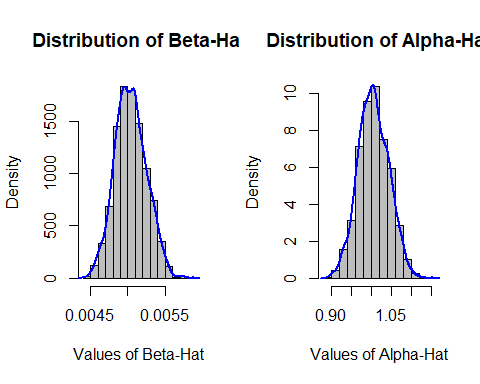
\includegraphics{Assignment_files/figure-latex/unnamed-chunk-12-1.pdf}

Based on the histograms and density plots for both estimators, the
distribution of β\^{}MOM and α\^{}MOM appears to be consistent with the
expectations from Question 8.

For the β\^{}MOM estimator, the distribution appears to be concentrated
around the mean value of approximately 0.005 and slightly right-skewed,
as anticipated. The density plot shows a somewhat flatter distribution
compared to a normal distribution, which is consistent with the negative
kurtosis mentioned earlier.

For the α\^{}MOM estimator, the distribution is also concentrated around
the mean value, which is close to 1. The histogram and density plot
reveal that the distribution is fairly symmetric, as expected, with a
shape similar to a normal distribution. This is in line with the
near-zero skewness and kurtosis calculated earlier.

In conclusion, the distribution of both estimators matches the
expectations based on the summary statistics and analysis in Question 8.
The β\^{}MOM estimator has a slightly skewed and flatter distribution,
while the α\^{}MOM estimator has a more symmetric and normal-like
distribution.

{ 10. Calculate the Coefficient of Variation (CV) for each estimator
(\(\hat{\alpha}\) and \(\hat{\beta}\)). Which estimator has the larger
relative variation?}

\begin{Shaded}
\begin{Highlighting}[]
\CommentTok{\# Calculate the CV for beta}
\FunctionTok{cv}\NormalTok{(betahat)}
\end{Highlighting}
\end{Shaded}

\begin{verbatim}
## [1] 0.04170685
\end{verbatim}

\begin{Shaded}
\begin{Highlighting}[]
\CommentTok{\# Calculate the CV for alpha}
\FunctionTok{cv}\NormalTok{(alphahat)}
\end{Highlighting}
\end{Shaded}

\begin{verbatim}
## [1] 0.0377303
\end{verbatim}

The coefficient of variation (CV) is calculated for each estimator
(α\^{}MOM and β\^{}MOM) to measure the relative variability of the
estimators. The CV is the ratio of the standard deviation to the mean,
expressed as a percentage. The results are as follows:

\begin{itemize}
\tightlist
\item
  CV for β\^{}MOM: 0.04170685 (approximately 4.17\%)
\item
  CV for α\^{}MOM: 0.0377303 (approximately 3.77\%)
\end{itemize}

Based on these results, the β\^{}MOM estimator has a larger relative
variation compared to the α\^{}MOM estimator. This means that the
β\^{}MOM estimator shows more variability relative to its mean value
compared to the α\^{}MOM estimator. In practical terms, this indicates
that the precision of the β\^{}MOM estimator is slightly lower than that
of the α\^{}MOM estimator.

{ 11. If you had a larger sample size in Question 4 (the value in the
size option of the code), how would you expect the distribution of your
estimators to change? }

If a larger sample size was used in Question 4, the distribution of the
estimators would likely become more concentrated around the true
parameter values. As the sample size increases, the precision of the
estimators generally improves, which results in a smaller standard
deviation and narrower distribution for both α\^{}MOM and β\^{}MOM.
Additionally, the central limit theorem implies that, with larger sample
sizes, the distribution of the estimators would tend to be closer to a
normal distribution, provided the underlying population is not highly
skewed or has extreme outliers.

{ 12. If you had a smaller number of REPLICATIONS in Question 4 (the
value after ``i in 1:zzzz''), how would you expect the distribution of
your estimators to change? }

If a smaller number of replications were used in Question 4, the
distribution of the estimators would be less stable and potentially less
accurate in approximating the true parameter values. This is because a
smaller number of replications means that fewer samples are used to
calculate the estimators, leading to greater variability and uncertainty
in the resulting distribution of the estimators. Consequently, the
standard deviation might be larger, and the distribution of the
estimators might deviate more from normality.

{ 13. The above analysis (Questions 4 - 10) is a statistical technique
called bootstrapping. Using this analysis, in your own words, define
bootstrapping and outline the basic steps of this technique. }

Bootstrapping is a resampling-based statistical technique used to
estimate the sampling distribution of a statistic by repeatedly drawing
samples (with replacement) from the original data and calculating the
statistic of interest for each resampled dataset. The basic steps of
bootstrapping are as follows: 1. Obtain an original sample from the
population.

\begin{enumerate}
\def\labelenumi{\arabic{enumi}.}
\setcounter{enumi}{1}
\item
  Draw a random sample with replacement from the original sample,
  keeping the sample size the same as the original sample.
\item
  Calculate the statistic of interest (e.g., mean, median, standard
  deviation, etc.) for the resampled dataset.
\item
  Repeat steps 2 and 3 a large number of times (e.g., 1,000 or 10,000
  replications) to obtain a large set of the statistic of interest.
\item
  Analyze the distribution of the statistic obtained from the resampled
  datasets, which approximates the sampling distribution of the
  statistic. This can be used to estimate confidence intervals, standard
  errors, or other measures of uncertainty for the statistic of
  interest.
\end{enumerate}

Bootstrapping is particularly useful when the underlying population
distribution is unknown, or when the sample size is small, making it
difficult to rely on parametric methods or traditional statistical
techniques.

\end{document}
